\documentclass[14pt, oneside]{altsu-report}

\worktype{Отчёт по практике на тему:}
\title{Разработка собственной игры на игровом Движке Godot}
\author{К.\,Д.~Сафронов }
\groupnumber{565}
\GradebookNumber{1337}
\supervisor{И.\,А.~Шмаков}
\supervisordegree{к.ф.-м.н., доцент}
\ministry{Министерство науки и высшего образования}
\country{Российской Федерации}
\fulluniversityname{ФГБОУ ВО Алтайский государственный университет}
\institute{Институт цифровых технологий, электроники и физики}
\department{Кафедра вычислительной техники и электроники}
\departmentchief{И.\,А.~Шмаков}
\departmentchiefdegree{ст. преп. каф. ВТиЭ}
\shortdepartment{ВТиЭ}
\abstractRU{Большой текст на русском! Пока счётчик работает не правильно! Поправьте количество рисунков и таблиц в cls-файле.}
\abstractEN{Большой текст на английском!}
\keysRU{компьютерное моделирование, cистема управления версиями}
\keysEN{computer simulation, distributed version control}

\date{\the\year}

% Подключение файлов с библиотекой.
\addbibresource{graduate-students.bib}

% Пакет для отладки отступов.
%\usepackage{showframe}

\begin{document}
\maketitle

\setcounter{page}{2}
\makeabstract
\tableofcontents

\chapter*{Введение}
\phantomsection\addcontentsline{toc}{chapter}{ВВЕДЕНИЕ}

\textbf{Актуальность:}
Актуальность разработки игр на движке Godot зависит от потребностей конкретного проекта и уровня опыта разработчика. Godot продолжает активно развиваться и улучшаться, привлекая все больше пользователей своими возможностями и гибкостью. В целом, Godot является конкурентоспособным инструментом для создания игр, особенно для небольших и средних проектов.

\textbf{Цель}
Научится работать с "Godot" и написать свою первую игру.

\textbf{Задачи:}
\begin{enumerate}
\item Исследовать основные принципы разработки игр на движке "Godot".
\item Изучить процесс проектирования, программирования и оптимизации игрового проекта.
\item Создать собственную игру с использованием данного движка.
\end{enumerate}

% Подключение первой главы (теория):
\chapter{\label{ch:ch01}ГЛАВА 1: Что такое <<Godot>>} % Нужно сделать главу в содержании заглавными буквами
\textbf{Godot Engine} (читается <<Годо>>)--- это открытый кроссплатформенный 2D и 3D игровой движок под лицензией MIT (это лицензия сбододного программного обеспечения, разработанная Массачусетским технологическим институтом), который разрабатывается сообществом Godot Engine Community. До публичного релиза в виде открытого ПО движок использовался внутри некоторых компаний Латинской Америки. Запускается среда разработки на Android, HTML5, Linux, macOS, Windows, BSD и Haiku, И может экспортировать игровые проекты на Пк, консоли, мобильные и веб-платформы.

\section{\label{sec:ch01/sec01}Раздел 1: Что такое игровые движки и какие есть?}
Игровой движок - это программное обеспечение, которое предоставляет разработчикам инструменты и функционал для создания и разработки видеоигр. Он представляет собой набор библиотек, инструментов, редакторов и других компонентов, которые облегчают процесс создания игр и позволяют разработчикам сосредоточиться на креативной части проекта, не тратя много времени на написание низкоуровневого кода.
Основные компонента игрового движка включает в себя:
\begin{itemize}
    \item Графический движок: Обеспечивает отображение графики, работу с 2D и 3D графикой, анимацией персонажей, освещением, эффектами и другими визуальными аспектами игры.
    \item Физический движок: Позволяет моделировать физические законы в игре, такие как гравитация, столкновения объектов, силы и т.д.
    \item Аудио---движок: Обеспечивает воспроизведение звуков и музыки в игре, управление звуковыми эффектами, микширование звука и другие аспекты аудио-дизайна.
    \item Инструменты разработки: Включают в себя редакторы уровней, ресурсов, скриптов, анимаций, а также другие инструменты для управления проектом и создания контента.
    \item Скриптовые языки:  Многие игровые движки предоставляют возможность программировать игровую логику с помощью скриптовых языков (например, C sharp, JavaScript, Python), что делает процесс разработки более гибким и доступным для широкого круга разработчиков.
\end{itemize}

На данный момент список самых популярных движков выглядит примерно так:
\begin{enumerate}
    \item Unity
    \item Unreal Engine
    \item Godot
    \item CryEngine
    \item GameMaker Studio
\end{enumerate}


\subsection{\label{subsec:ch01/sec01/sub01}Отличие Godot от остальных}
Немного о самом популярном движке Unity, а также его отличие от Godot:
Unity--- тоже кроссплатформенная среда разработки компьютерных игр, разработанная американской компанией Unity Technologies.Основными преимуществами Unity являются наличие визуальной среды разработки, межплатформенной поддержки и модульной системы компонентов. К недостаткам относят появление сложностей при работе с многокомпонентными схемами и затруднения при подключении внешних библиотек.На Unity написаны тысячи игр, приложений, визуализации математических моделей, которые охватывают множество платформ и жанров. При этом Unity используется как крупными разработчиками, так и независимыми студиями.


Основные отличия <<Godot>> и <<Unity>>:
\begin{enumerate}
\item Лицензирование:
    \begin{itemize}
        \item <<Godot>>: Godot распространяется под лицензией MIT, что означает, что его можно использовать бесплатно как для коммерческих, так и для некоммерческих проектов без необходимости платить роялти (это плата, которую разработчики или авторы должны выплачивать владельцам прав на использование их интеллектуальной собственности. В контексте игровой индустрии платить роялти означает, что разработчики должны выплачивать определенный процент от выручки или прибыли от продаж игры или другого продукта владельцу игрового движка, платформы или другому правообладателю).
        \item <<Unity>>: Unity имеет различные версии, включая бесплатную версию (Personal Edition) и платные версии с дополнительными функциями. При этом есть ограничения на доходы, полученные от проекта.
    \end{itemize}
\item Язык программирования:
    \begin{itemize}
        \item <<Godot>>: В Godot используется собственный язык программирования GDScript, который похож на Python. Также поддерживаются C sharp и VisualScript.
        \item <<Unity>>: Unity обычно использует C sharp в качестве основного языка программирования, но также поддерживает JavaScript и Boo.
    \end{itemize}
\item Редактор:
    \begin{itemize}
        \item <<Godot>>: Редактор Godot имеет интуитивно понятный интерфейс и обладает множеством инструментов для создания игр, включая редактор уровней, анимаций, ресурсов и скриптов.
        \item <<Unity>>: Unity также предоставляет мощный редактор с широким спектром возможностей, включая создание игровых объектов, компонентов, анимаций и других элементов.
    \end{itemize}
\item Системы физики:
    \begin{itemize}
        \item <<Godot>>: Godot имеет встроенную физическую систему, которая позволяет моделировать физические законы в игре.
        \item <<Unity>>: Unity также имеет свою физическую систему, которая предоставляет возможности моделирования столкновений, гравитации и других физических эффектов.
    \end{itemize}
\item Сообщество и поддержка:
    \begin{itemize}
        \item <<Godot>>: Сообщество Godot активно развивается и предоставляет множество ресурсов, учебных материалов и документации для разработчиков.
        \item <<Unity>>: Unity имеет огромное сообщество разработчиков, множество плагинов и активную поддержку со стороны компании.
    \end{itemize}
\end{enumerate}
Оба движка имеют свои преимущества и недостатки, и выбор между ними зависит от конкретных потребностей проекта и личных предпочтений разработчика.


\section{\label{sec:ch01/sec02}Чем же Godot и Unity различаются}
Так как мы рассмотрели основные отличия этих двух замечательных движков, логично будет разобрать и их сходства:
\begin{enumerate}
    \item  Мультиплатформенность: Оба движка поддерживают разработку игр для различных платформ, таких как Windows, macOS, Linux, iOS, Android и другие.
    \item Визуальные редакторы:  У обоих движков есть визуальные редакторы, которые позволяют создавать игровые сцены, анимации, интерфейсы и другие элементы без необходимости писать код.
    \item Языки программирования: Оба движка поддерживают несколько языков программирования для разработки игр. Например, Godot использует свой собственный язык GDScript, а Unity поддерживает C sharp, JavaScript и Boo.
    \item Сообщество и документация: У обоих движков активные сообщества разработчиков и обширная документация, что облегчает изучение и использование движков.
    \item Ресурсы и активы: Оба движка имеют магазины активов (Asset Stores), где разработчики могут приобрести готовые ресурсы, такие как модели, текстуры, звуки и другие элементы для использования в своих проектах.
\end{enumerate}


Пример вложенного нумерованного списка:
\begin{enumerate}
\item Первый элемент:
\begin{enumerate}
\item Первый элемент первого элемента;
\item Второй элемент первого элемента;
\end{enumerate}
\item Второй элемент:
\begin{enumerate}
\item Первый элемент второго элемента;
\item Второй элемент второго элемента.
\end{enumerate}
\end{enumerate}

\section{\label{sec:ch01/sec03}Системные требования }

Требования <<Godot>>~\ref{tab:example01}.
\begin{table}[H]
\caption{\centering\label{tab:example01}Системные требования <<Godot>>}
\begin{tabular}{|p{3 cm}|p{5 cm}|}
\hline
Версия операционной системы & Windows 7 SP1+, macOS 10.11+, Linux \\ \hline
Процессор & 64-битный двухъядерный процессор, тактовая частота 2.0 ГГц+ \\ \hline
Графический API & с поддержкой OpenGL ES 3.0+ \\ \hline
Свободное место & 1 ГБ+ \\ \hline
Оперативная память & 2 ГБ \\ \hline
\end{tabular}
\end{table}

Системные требования <<Unity>>~\ref{tab:example02}.
\begin{table}[H]
\caption{\centering\label{tab:example02}Системные требования <<Unity>>}
\begin{tabular}{|p{3 cm}|p{5 cm}|}
\hline
Версия операционной системы & Windows 7 SP1+, 8, 10, macOS 10.12+ \\ \hline
Процессор & поддержка SSE2 \\ \hline
Графический API & с поддержкой DirectX 11 или Metal \\ \hline
Свободное место & 10 GB свободного места \\ \hline
Оперативная память & 4 ГБ \\ \hline
\end{tabular}
\end{table}
\par
Требования, что были указаны выше, являются минимальными для работы с данными движками.
% Подключение второй главы (практическая часть):
\chapter{\label{ch:ch02}ГЛАВА 2: Знакомство с интерфейсом <<Godot>>}

\section{\label{sec:ch02/sec01}Установка <<Godot>>}

\subsection{\label{subsec:ch02/sec01/sub01}Переход на сайт}
Установить наш движок мы можем несколькими методами:
\begin{itemize}
    \item Через Steam
    \item Через официальный сайт
\end{itemize}


\begin{figure}[h]
    \centering
    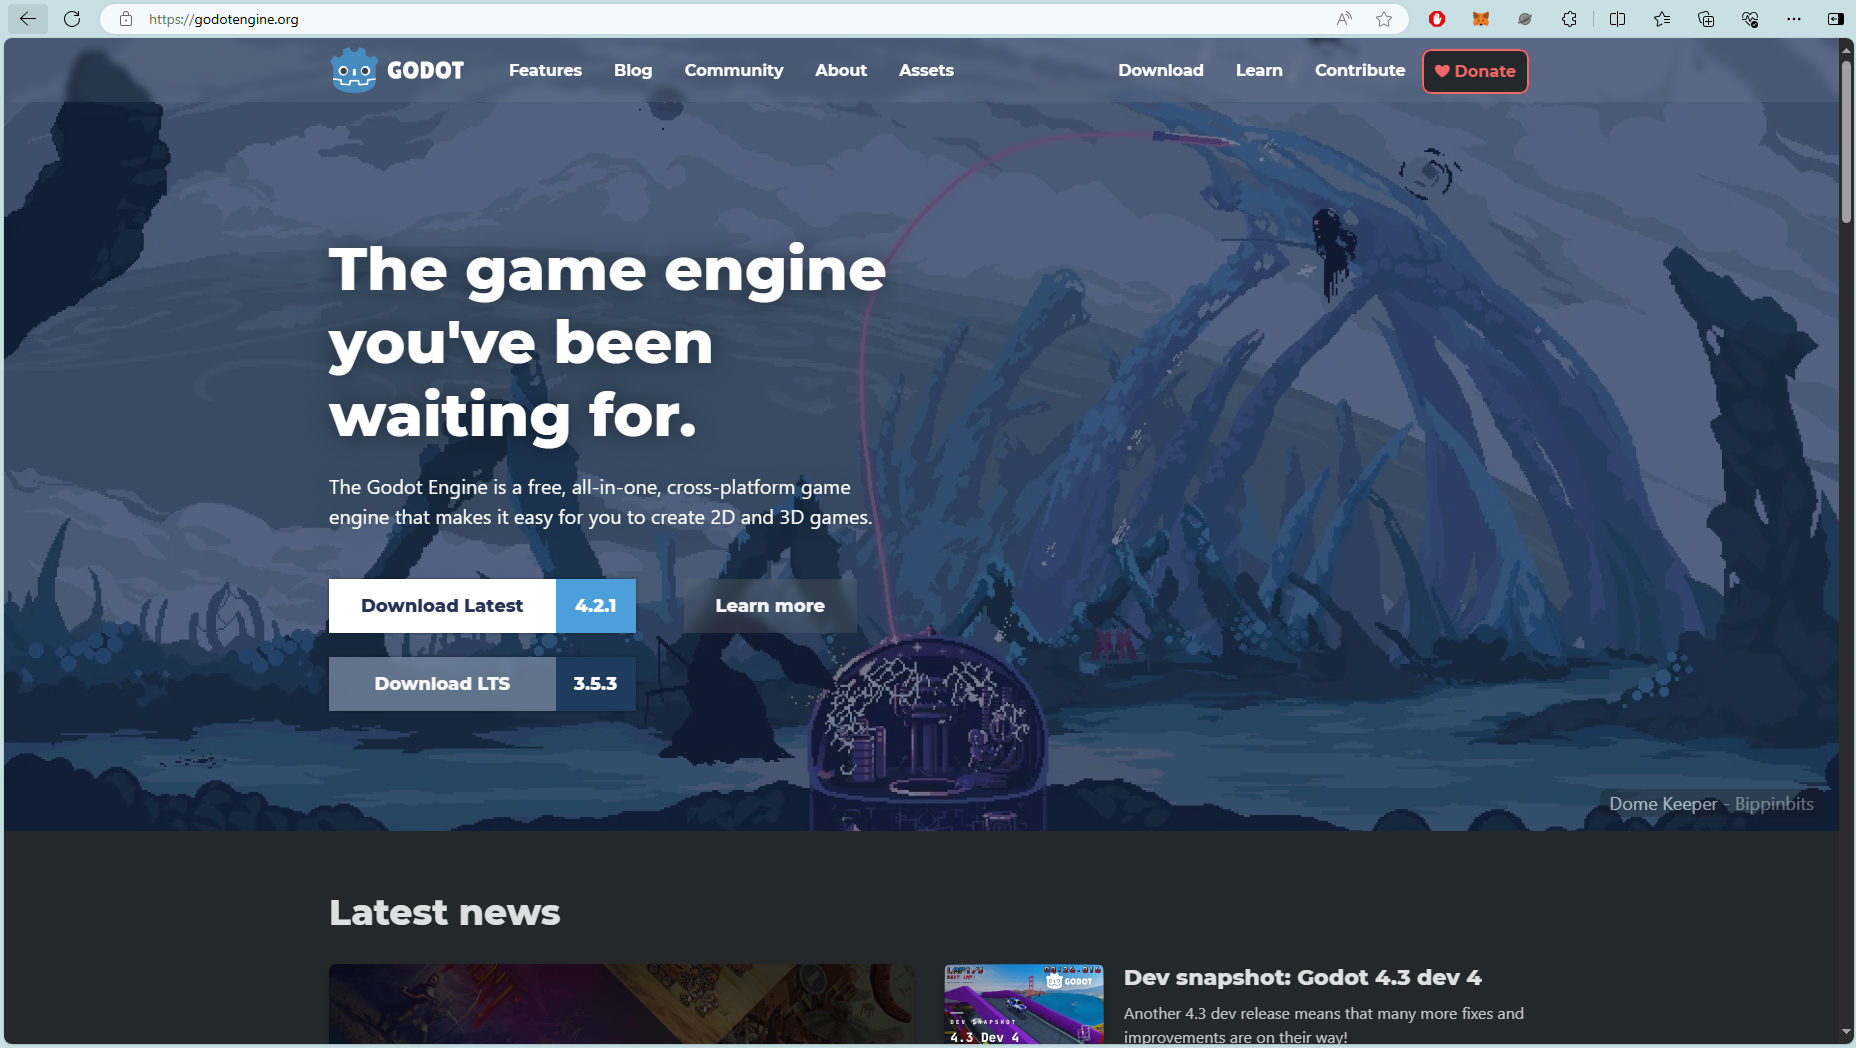
\includegraphics[width=1\textwidth]{images/godotsait.png}
\caption{\centering\label{fig:example03}Официальный сайт <<Godot>>.}
\end{figure}


\begin{figure}[h]
    \centering
    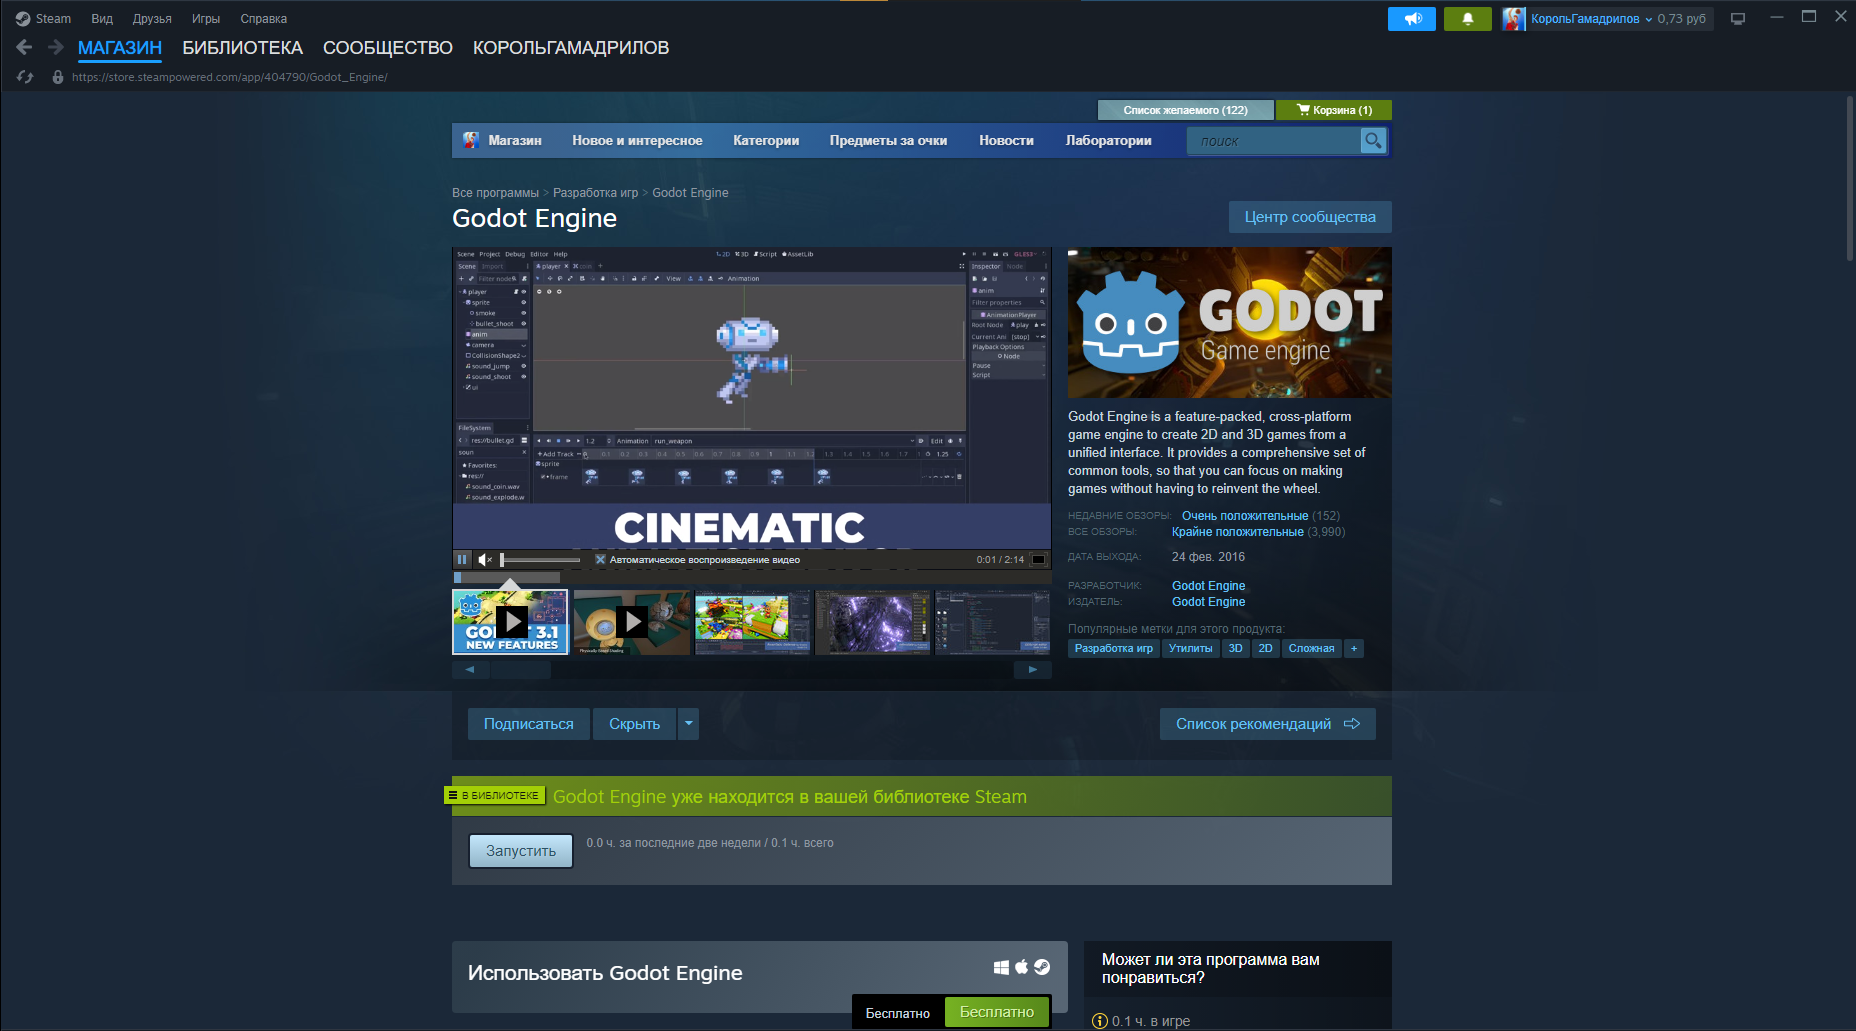
\includegraphics[width=1\textwidth]{images/godotSteam.png}
\caption{\centering\label{fig:example04}Официальная страница <<Godot>> в Steam.}
\end{figure}


\subsection{\label{subsec:ch02/sec02/sub01}Создание проекта}
Как только мы установили <<Godot>> на наш пк, мы открываем его и вот что нас встречает:
\section{\label{sec:ch02/sec02}Интерфейс программы}

\begin{figure}[h]
    \centering
    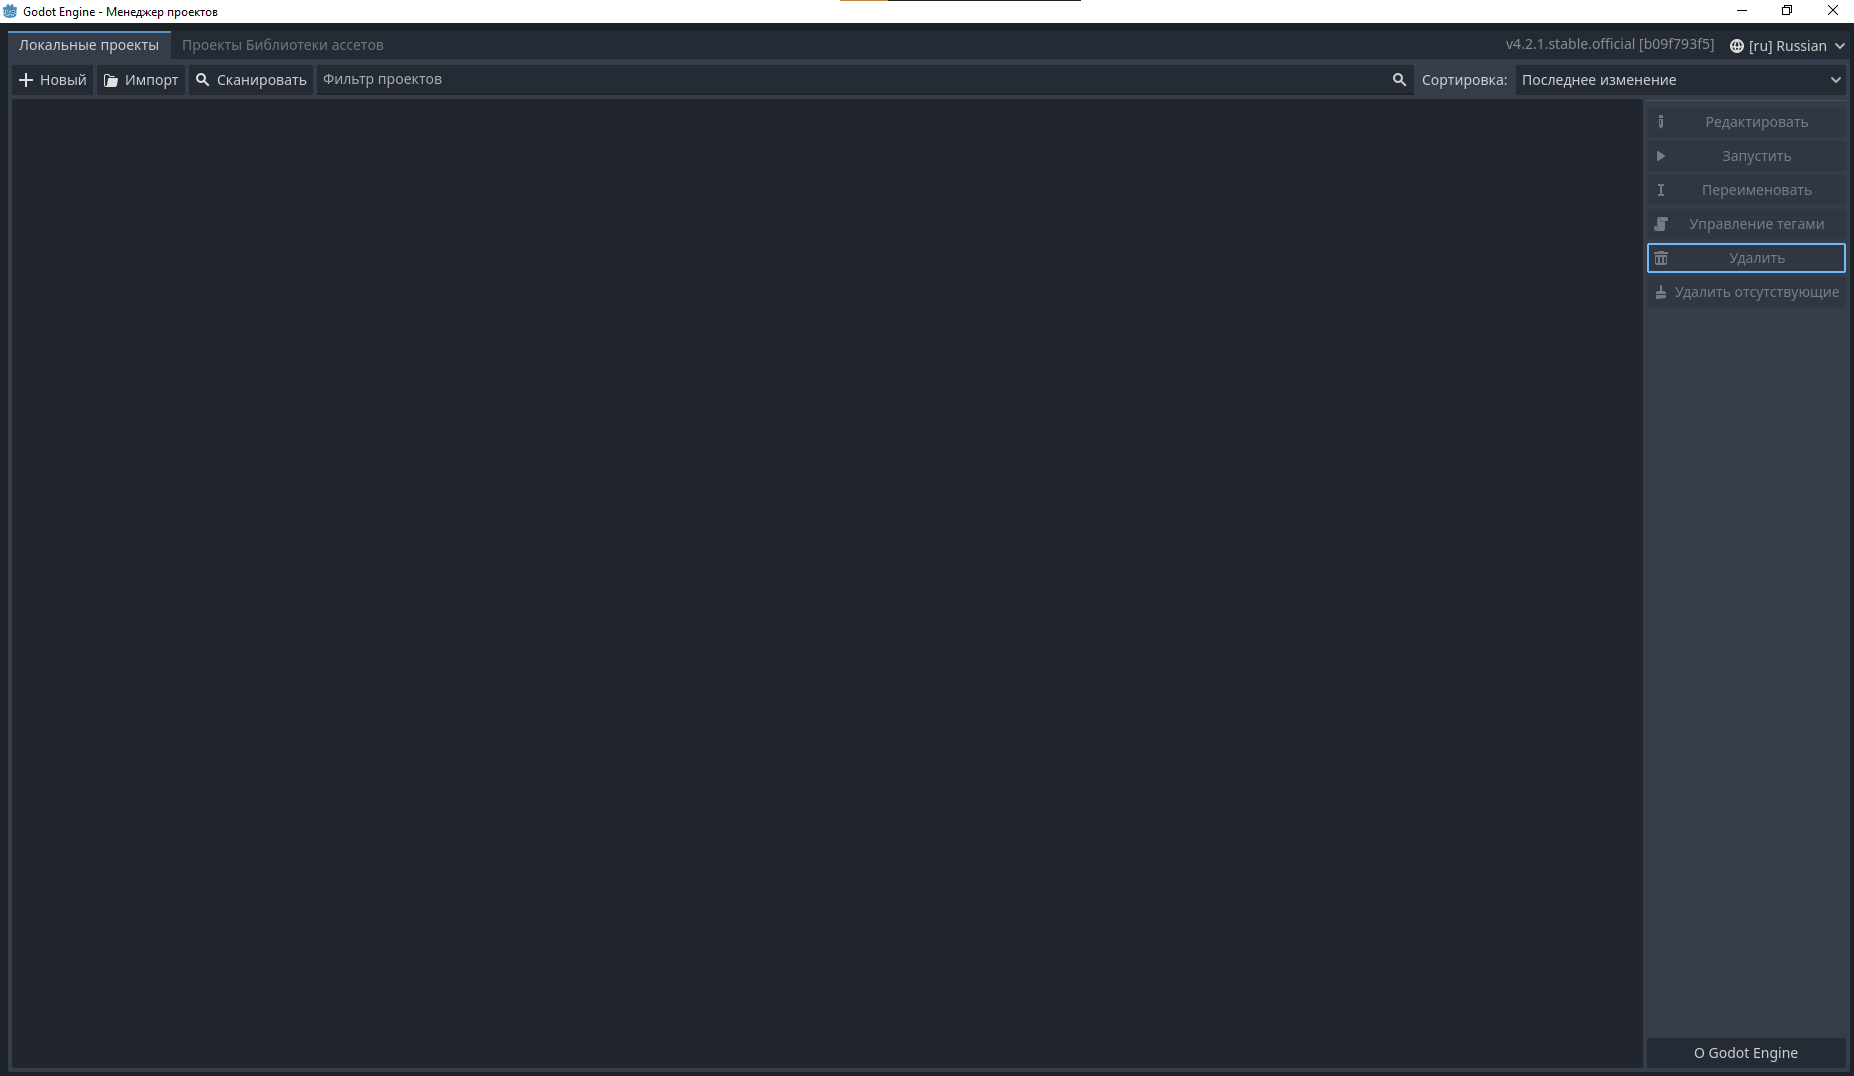
\includegraphics[width=1\textwidth]{images/Менеджер проектов.png}
\caption{\centering\label{fig:example05}Менеджер проектов.}
\end{figure}

% Подключение третий главы (практическая часть с тестированием:
\chapter{\label{ch:ch03}ГЛАВА 3}

Пример ссылок:
\begin{enumerate}
\item на главу~\ref{ch:ch01};
\item на раздел~\ref{sec:ch01/sec01} главы~\ref{ch:ch01};
\item на раздел~\ref{sec:ch02/sec01} главы~\ref{ch:ch02};
\item на приложение на странице~\pageref{appendix1};
\item на код на странице~\pageref{code:pi-example}.
\end{enumerate}

\section{\label{sec:ch03/sec01}Раздел 1}

\subsection{\label{subsec:ch03/sec01/sub01}Подраздел 1}

\subsection{\label{subsec:ch03/sec01/sub02}Подраздел 2}

\section{\label{sec:ch03/sec02}Раздел 2}

\subsection{\label{subsec:ch03/sec02/sub01}Подраздел 1}

\subsection{\label{subsec:ch03/sec02/sub02}Подраздел 2}

Пример ссылки на рисунок в документе~\ref{fig:example05}.
\begin{figure}[h]
    \centering
    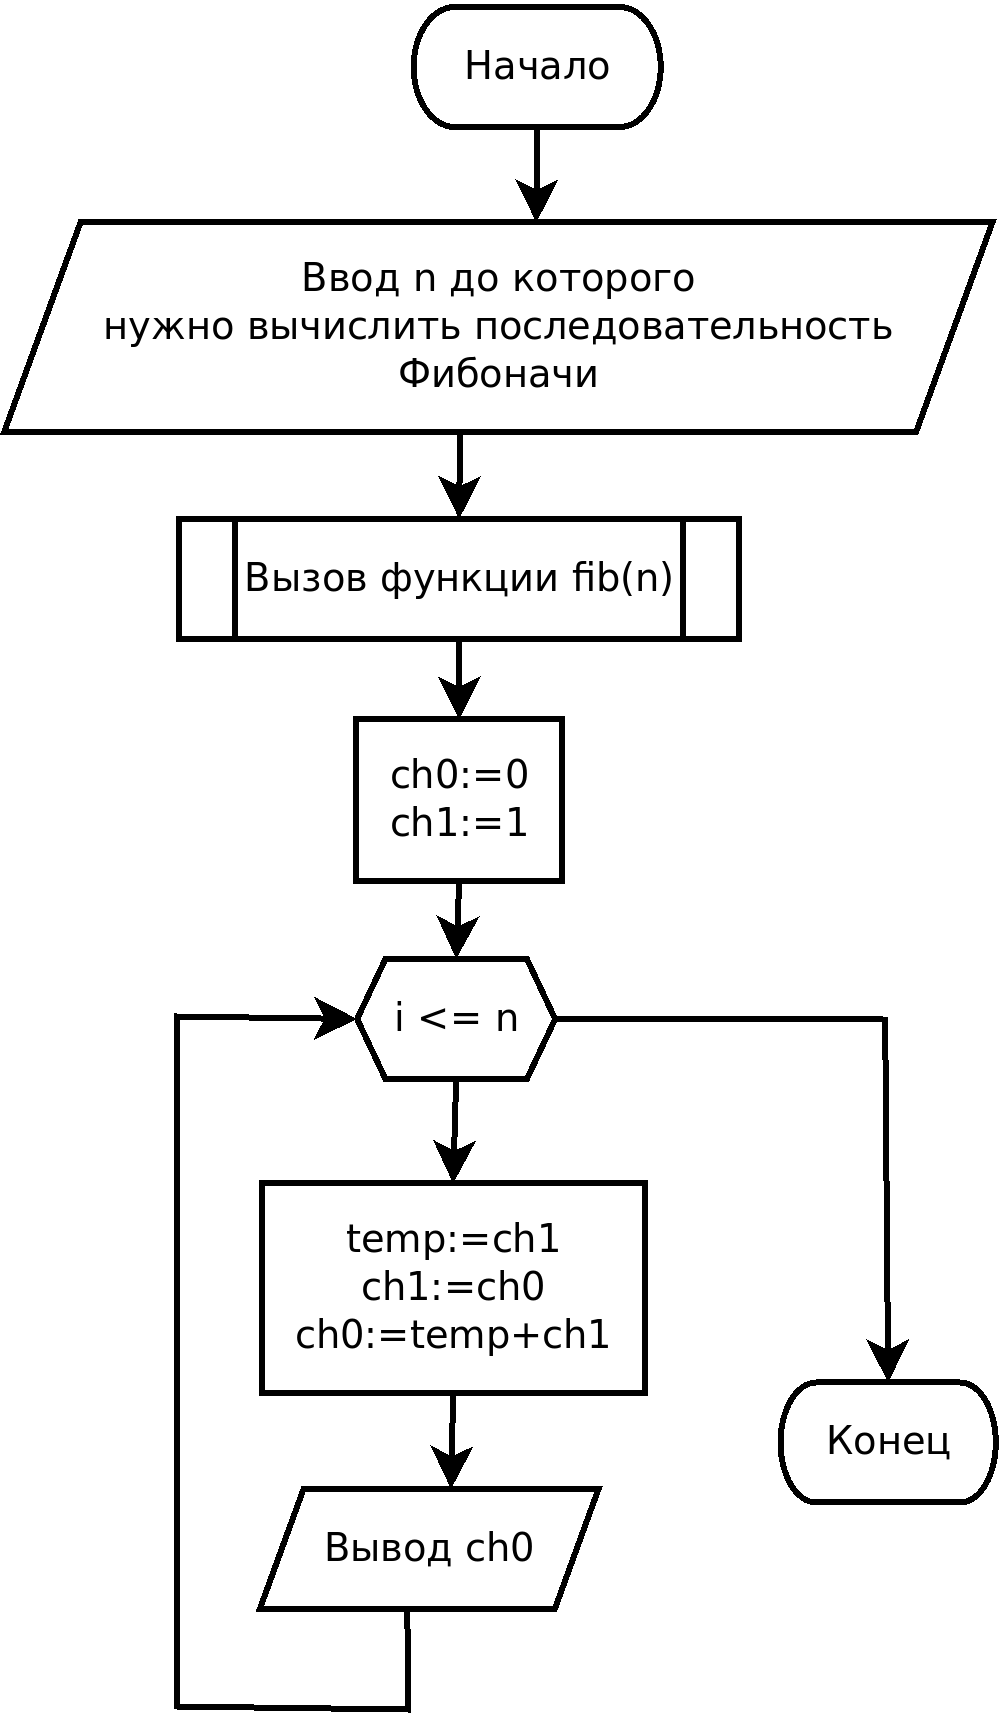
\includegraphics[width=0.5\textwidth]{./images/fibonacci.png}
    \caption{\centering\label{fig:example05}Пример рисунка в формате PNG.}
\end{figure}

Пример ссылки на рисунок в документе~\ref{fig:example06}.
\begin{figure}[h]
    \centering
    \includesvg[width=0.5\textwidth]{./images/fibonacci.svg}
    \caption{\centering\label{fig:example06}Пример рисунка в формате SVG.}
\end{figure}

Пример ссылки на таблицу в документе~\ref{tab:example05}.
\begin{table}[H]
\caption{\centering\label{tab:example05}Системные требования}
\begin{tabular}{|p{3 cm}|p{3 cm}|p{3 cm}|p{5 cm}|}
\hline
Минимальные требования & 1 & 2 & 3 \\ \hline
Версия операционной системы & 1 & 2 & 3 \\ \hline
Процессор & 1 & 2 & 3 \\ \hline
Графический API & 1 & 2 & 3 \\ \hline
\end{tabular}
\end{table}

Пример ссылки на таблицу в документе~\ref{tab:example06}.
\begin{table}[H]
\caption{\centering\label{tab:example06}Системные требования}
\begin{tabular}{|p{3 cm}|p{3 cm}|p{3 cm}|p{5 cm}|}
\hline
Минимальные требования & 1 & 2 & 3 \\ \hline
Версия операционной системы & 1 & 2 & 3 \\ \hline
Процессор & 1 & 2 & 3 \\ \hline
Графический API & 1 & 2 & 3 \\ \hline
\end{tabular}
\end{table}

Пример использования minted для оформления кода и ссылка на этот код~\ref{code:example05}.
\begin{code}
\captionof{listing}{\centering\label{code:example05}Вычисление последовательности Фибоначчи}
\vspace{-\baselineskip}\begin{minted}{C}
#include <stdio.h>
#include <omp.h>
#define N 100

int main(int argc, char *argv[]) {
  double a[N], b[N], c[N];
  int i;
  omp_set_dynamic(0); // запретить библиотеке openmp менять число потоков во время исполнения
  omp_set_num_threads(10); // установить число потоков в 10
  // инициализируем массивы
  for (i = 0; i < N; i++) {
      a[i] = i * 1.0;
      b[i] = i * 2.0;
  }
  // вычисляем сумму массивов
#pragma omp parallel for shared(a, b, c) private(i)
   for (i = 0; i < N; i++)
     c[i] = a[i] + b[i];

  printf ("%f\n", c[10]);
  return 0;
}
\end{minted}
\end{code}

Пример использования minted для оформления кода и ссылка на этот код~\ref{code:example06}.
\begin{code}
\captionof{listing}{\centering\label{code:example06}Сложение двух массивов параллельно десятью потоками (пример из https://ru.wikipedia.org/wiki/OpenMP)}
\vspace{-\baselineskip}\begin{minted}{C}
#include <stdio.h>
#include <omp.h>
#define N 100

int main(int argc, char *argv[]) {
  double a[N], b[N], c[N];
  int i;
  omp_set_dynamic(0); // запретить библиотеке openmp менять число потоков во время исполнения
  omp_set_num_threads(10); // установить число потоков в 10
  // инициализируем массивы
  for (i = 0; i < N; i++) {
      a[i] = i * 1.0;
      b[i] = i * 2.0;
  }
  // вычисляем сумму массивов
#pragma omp parallel for shared(a, b, c) private(i)
   for (i = 0; i < N; i++)
     c[i] = a[i] + b[i];

  printf ("%f\n", c[10]);
  return 0;
}
\end{minted}
\end{code}


\chapter*{Заключение}
\phantomsection\addcontentsline{toc}{chapter}{ЗАКЛЮЧЕНИЕ}

\begin{enumerate}
\item Пример ссылки на электронный источник~\cite{wikiRUBitbucket,wikiRUIdSoftware,wikiRUGitHub}.
\item Пример ссылки на книгу одного автора~\cite{book1author}.
\item Пример ссылки на книгу 5-ти и более авторов~\cite{book5author}.
\end{enumerate}

\newpage
\phantomsection\addcontentsline{toc}{chapter}{СПИСОК ИСПОЛЬЗОВАННОЙ ЛИТЕРАТУРЫ}
\printbibliography[title={Список использованной литературы}]

\appendix
\newpage
\chapter*{\raggedleft\label{appendix1}Приложение}
\phantomsection\addcontentsline{toc}{chapter}{ПРИЛОЖЕНИЕ}
%\section*{\centering\label{code:appendix}Текст программы}

\begin{center}
\label{code:appendix}Текст программы
\end{center}

\begin{code}
\captionof*{listing}{\centering\label{code:pi-example}Пример программы вычисления числа $\pi$ на языке \textit{C} с использованием \textit{MPI} (пример из https://ru.wikipedia
.org/wiki/Message\_Passing\_Interface)}
\vspace{-1cm}\inputminted{C}{src/pi-mpi.c}
\end{code}

\end{document}

